\documentclass[conference]{IEEEtran}

\usepackage[utf8]{inputenc}
\usepackage[T5]{fontenc}
\usepackage[vietnamese]{babel}
\usepackage{graphicx}
\usepackage{booktabs}
\usepackage{amsmath}
\usepackage{hyperref}
\usepackage{enumitem}
\usepackage{balance}

\graphicspath{{../reports/figures/}}

\title{An Explainable AI Framework for Telecom Customer Churn Prediction and SHAP-Based Retention Personas}

\author{
\IEEEauthorblockN{Vũ Trung Kiên}
\IEEEauthorblockA{Department of Data Science\\University of Information Technology\\Ho Chi Minh City, Vietnam\\Email: student@uit.edu.vn}
}

\begin{document}

\maketitle

\begin{abstract}
Customer churn prediction is a critical task in telecom because retaining existing customers is typically cheaper than acquiring new ones. This paper presents a three-layer explainable pipeline: churn prediction, SHAP-based explanation, and SHAP-driven customer segmentation for retention planning. Using the Telco Customer Churn dataset with 7,043 customers, we compare eight classification models and observe the trade-off between predictive performance and interpretability. Logistic Regression gives the highest accuracy and AUC, but Random Forest is selected as the base model because it integrates naturally with SHAP analysis. SHAP highlights Contract, tenure, OnlineSecurity, TechSupport, and TotalCharges as the strongest churn drivers. When clustering on theme-level SHAP representations, the best configuration reaches a silhouette score of 0.3157 with five clusters, improving by 5.16\% over raw-feature clustering. All four SHAP themes are statistically significant under Kruskal-Wallis, and the resulting personas map directly to targeted retention actions.
\end{abstract}

\begin{IEEEkeywords}
Customer churn, explainable AI, SHAP, clustering, telecom, retention.
\end{IEEEkeywords}

\section{Introduction}
Customer churn is one of the most costly issues for telecom providers. If a model only predicts whether a customer will leave, it remains difficult for business teams to translate that output into concrete retention plans. In practice, we need models that are not only accurate, but also explainable and actionable.

Traditional churn studies often optimize metrics such as accuracy or F1-score without answering why customers leave or how providers should intervene. To address this gap, this paper combines prediction, explanation, and segmentation into a single pipeline \cite{alam2020customer, lundberg2017unified, breiman2001random}.

\textbf{Main contributions}:
\begin{itemize}[leftmargin=*]
    \item A comparative churn modeling workflow with multiple classifiers and SHAP-compatible model selection.
    \item Global and local churn explanations using SHAP, with business-oriented interpretation of the strongest drivers.
    \item SHAP theme clustering to create retention personas and map each persona to an actionable retention strategy.
\end{itemize}

\section{Data and Preprocessing}
The study uses the public \emph{Telco Customer Churn} dataset, containing 7,043 customers and 21 original attributes. The churn rate is 26.54\% (1,869 churners), so the task is moderately imbalanced.

The preprocessing steps are:
\begin{itemize}[leftmargin=*]
    \item Convert \texttt{TotalCharges} to numeric and drop invalid rows.
    \item Remove \texttt{customerID}.
    \item Label-encode categorical variables.
    \item Engineer three features: \texttt{AvgMonthlyCharge}, \texttt{HighCharge}, and \texttt{LowTenureHighCharge}.
    \item Standardize \texttt{tenure}, \texttt{MonthlyCharges}, \texttt{TotalCharges}, and \texttt{AvgMonthlyCharge}.
    \item Split the data into train/test sets using an 80/20 stratified split.
\end{itemize}

After preprocessing, the training set contains 5,625 samples and the test set contains 1,407 samples.

\section{Methodology}
\subsection{Model Comparison}
Eight models are evaluated: Logistic Regression, Random Forest, Decision Tree, AdaBoost, linear SVM, KNN, Naive Bayes, and XGBoost. Performance is measured using accuracy, precision, recall, F1-score, and AUC.

\subsection{SHAP Explanation}
After model selection, SHAP is used to quantify each feature's contribution to churn probability. Mean absolute SHAP values are used for global ranking, and SHAP summary plots are used to inspect directionality of the effects \cite{lundberg2017unified}.

\subsection{Persona Clustering on SHAP Themes}
To convert explanations into action, SHAP features are grouped into four business themes:
\begin{itemize}[leftmargin=*]
    \item \textbf{Cost\_Pressure}: charges and payment pressure.
    \item \textbf{Commitment}: contract length and customer commitment.
    \item \textbf{Service\_Quality}: network quality and technical support.
    \item \textbf{Lifestyle\_Bundle}: entertainment and bundle preferences.
\end{itemize}

Because these themes may still be correlated, the theme space is standardized before KMeans clustering \cite{macqueen1967some}. The cluster count is selected using silhouette score. This design reduces multicollinearity among variables such as \texttt{Contract}, \texttt{tenure}, and \texttt{AvgMonthlyCharge} while preserving business meaning.

\section{Results}
\subsection{Model Comparison}
Table~\ref{tab:model_comparison_en} summarizes the eight models. Logistic Regression achieves the highest accuracy and AUC in this benchmark, while Naive Bayes gives the highest recall and F1 among the tested methods. Random Forest is not the best model numerically, but it is selected as the base model because it is well-suited to TreeExplainer-based SHAP analysis.

\begin{table}[t]
\centering
\caption{Model comparison}
\label{tab:model_comparison_en}
\resizebox{\columnwidth}{!}{%
\begin{tabular}{lccccc}
\toprule
Model & Accuracy & Precision & Recall & F1 & AUC \\
\midrule
Logistic Regression & 0.7903 & 0.6215 & 0.5401 & 0.5780 & 0.8359 \\
Random Forest & 0.7846 & 0.6172 & 0.5000 & 0.5524 & 0.8148 \\
Decision Tree & 0.7257 & 0.4845 & 0.5027 & 0.4934 & 0.6554 \\
AdaBoost & 0.7832 & 0.6062 & 0.5267 & 0.5637 & 0.8341 \\
SVM (Linear) & 0.7839 & 0.6562 & 0.3930 & 0.4916 & 0.8332 \\
KNN & 0.7697 & 0.5710 & 0.5374 & 0.5537 & 0.7826 \\
Naive Bayes & 0.7562 & 0.5332 & 0.6658 & 0.5922 & 0.8114 \\
XGBoost & 0.7854 & 0.6091 & 0.5374 & 0.5710 & 0.8174 \\
\bottomrule
\end{tabular}%
}
\end{table}

\subsection{SHAP Feature Importance}
SHAP identifies Contract as the most important feature, followed by tenure, OnlineSecurity, TechSupport, and TotalCharges. This is consistent with telecom intuition: commitment level and service quality strongly influence whether a customer stays.

\begin{table}[t]
\centering
\caption{Top 10 features by mean absolute SHAP}
\label{tab:shap_top10_en}
\resizebox{\columnwidth}{!}{%
\begin{tabular}{lcc}
\toprule
Rank & Feature & Mean $|$SHAP$|$ \\
\midrule
1 & Contract & 0.0794 \\
2 & tenure & 0.0497 \\
3 & OnlineSecurity & 0.0382 \\
4 & TechSupport & 0.0340 \\
5 & TotalCharges & 0.0326 \\
6 & InternetService & 0.0275 \\
7 & MonthlyCharges & 0.0253 \\
8 & OnlineBackup & 0.0184 \\
9 & AvgMonthlyCharge & 0.0154 \\
10 & PaymentMethod & 0.0151 \\
\bottomrule
\end{tabular}%
}
\end{table}

\begin{figure}[t]
\centering
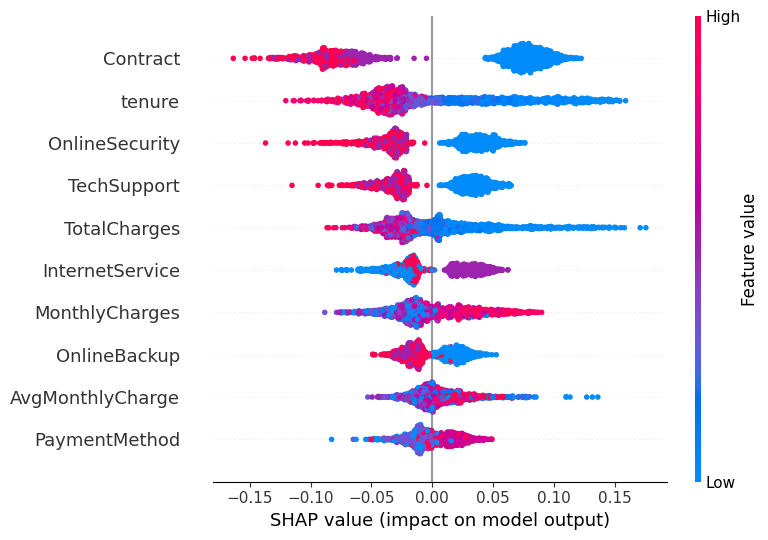
\includegraphics[width=\columnwidth]{shap_summary.png}
\caption{SHAP summary plot for the base model}
\label{fig:shap_summary_en}
\end{figure}

\subsection{Ablation Study for Clustering Spaces}
We compare three clustering spaces: raw features, per-feature SHAP values, and theme-level SHAP representations. Table~\ref{tab:ablation_en} shows that SHAP theme space provides the best clustering quality.

\begin{table}[t]
\centering
\caption{Ablation study for clustering spaces}
\label{tab:ablation_en}
\resizebox{\columnwidth}{!}{%
\begin{tabular}{lcccc}
\toprule
Space & Best k & Silhouette & Davies-Bouldin & Improvement vs. raw \\
\midrule
raw\_feature & 3 & 0.3002 & 1.3141 & - \\
shap\_value & 2 & 0.3073 & 1.5033 & 2.36\% \\
shap\_theme & 5 & 0.3157 & 1.0592 & 5.16\% \\
\bottomrule
\end{tabular}%
}
\end{table}

\begin{figure}[t]
\centering
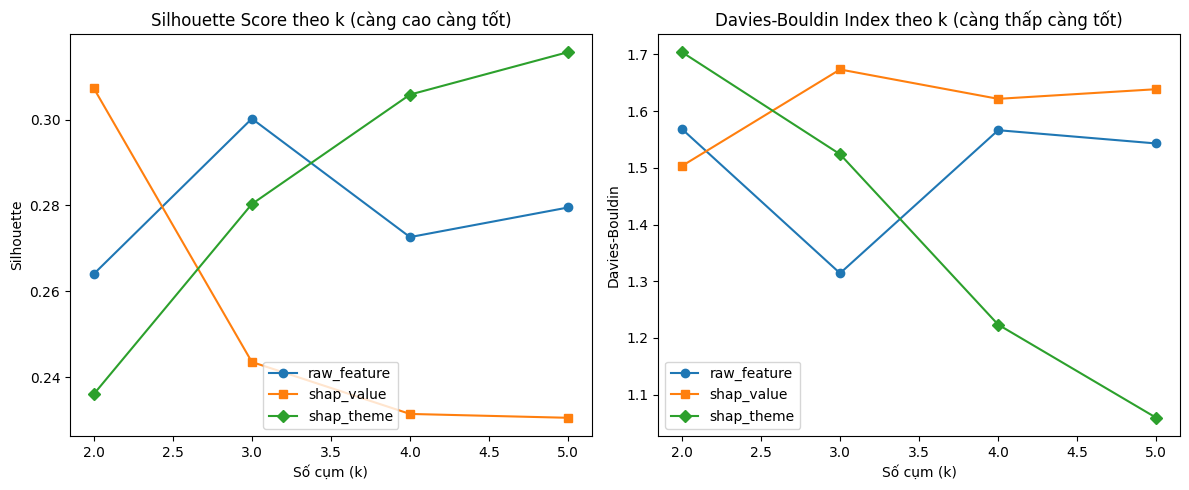
\includegraphics[width=\columnwidth]{ablation_raw_vs_shap.png}
\caption{Clustering quality comparison across three representation spaces}
\label{fig:ablation_en}
\end{figure}

This result shows that aggregating SHAP values into business themes is not only more interpretable, but also improves cluster separability. That matters because personas are useful only when they are distinct enough to support different retention actions.

\subsection{Personas and Retention Recommendations}
Clustering on SHAP themes produces five personas with sizes 230, 582, 237, 225, and 133. All four themes show statistically significant differences between personas, with large effect sizes under the Kruskal-Wallis test (100\% significant at $p<0.05$). This confirms that the clusters are not random artifacts.

\begin{table}[t]
\centering
\caption{Persona summary and retention actions}
\label{tab:persona_en}
\resizebox{\columnwidth}{!}{%
\begin{tabular}{cllcp{2.7cm}}
\toprule
ID & Size & Main theme & Distinctive feature & Retention action \\
\midrule
0 & 230 & Service\_Quality & OnlineSecurity & Strengthen technical support, improve network quality, and provide post-sales care \\
1 & 582 & Commitment & Contract & Offer long-term contract incentives and staged retention programs \\
2 & 237 & Service\_Quality & InternetService & Strengthen technical support, improve network quality, and provide post-sales care \\
3 & 225 & Lifestyle\_Bundle & - & Offer discounted bundles for streaming and multiple-line services \\
4 & 133 & Cost\_Pressure & TotalCharges & Provide fee reductions, vouchers, or flexible plans \\
\bottomrule
\end{tabular}%
}
\end{table}

The largest persona is the commitment-sensitive group, which aligns with the churn-by-contract distribution: month-to-month customers churn at 0.427, compared with 0.113 for one-year contracts and 0.028 for two-year contracts. This supports the interpretation that Contract is not only the strongest SHAP feature, but also a compact proxy for customer commitment and switching cost.

\subsection{Overall Interpretation}
The results suggest three practical conclusions:
\begin{itemize}[leftmargin=*]
    \item Churn in this dataset is strongly driven by commitment and contract structure.
    \item Service quality and cost pressure are the two most actionable business themes for retention design.
    \item SHAP theme clustering yields personas that are more meaningful than clustering on raw features alone.
\end{itemize}

\section{Conclusion}
This paper presents an explainable churn framework that can be translated into concrete telecom retention actions. Rather than stopping at prediction, the proposed workflow connects prediction, explanation, and persona segmentation. On the Telco Customer Churn dataset, the pipeline identifies the key churn drivers, produces five distinct personas, and maps them to targeted retention strategies.

Future work can incorporate behavioral time-series data, experiment with additional clustering strategies, and evaluate the business impact of each retention policy on real-world customers.

\balance

\bibliographystyle{IEEEtran}
\bibliography{references}

\end{document}
